%\documentclass[aspectratio=169, handout]{beamer}
\documentclass[aspectratio=169]{beamer}


\makeatletter
\renewcommand*\env@matrix[1][\arraystretch]{%
  \edef\arraystretch{#1}%
  \hskip -\arraycolsep
  \let\@ifnextchar\new@ifnextchar
  \array{*\c@MaxMatrixCols c}}
\makeatother

\usepackage{tikz}
\usetikzlibrary{tikzmark,fit,shapes.geometric}

\newcommand{\transp}{^{\rm{T}}}

\usepackage{cases}
\usepackage[english]{babel}
% or whatever
\usepackage{xcolor}
\usepackage{colortbl}
\usepackage[latin1]{inputenc}
\usepackage[super]{nth}
% or whatever
%\setbeamertemplate{footline}[page number]
\setbeamertemplate{footline}
        {
      \leavevmode%
      \hbox{%
      \begin{beamercolorbox}[wd=.333333\paperwidth,ht=2.25ex,dp=1ex,center]{author in head/foot}%
        \usebeamerfont{author in head/foot}\insertshortauthor%~~(\insertshortinstitute)
      \end{beamercolorbox}%
      \begin{beamercolorbox}[wd=.333333\paperwidth,ht=2.25ex,dp=1ex,center]{title in head/foot}%
        \usebeamerfont{title in head/foot}\insertshorttitle
      \end{beamercolorbox}%
      \begin{beamercolorbox}[wd=.333333\paperwidth,ht=2.25ex,dp=1ex,right]{date in head/foot}%
        \usebeamerfont{date in head/foot}\insertshortdate{}\hspace*{2em} \insertframenumber{}  \hspace*{2em}%/ \inserttotalframenumber\hspace*{2ex} 

    %#turning the next line into a comment, erases the frame numbers
        

      \end{beamercolorbox}}%
      \vskip 0pt%
    }

\usepackage{times}
\usepackage[T1]{fontenc}
\usepackage{psfrag}
\usepackage{algorithm}
\usepackage{amsmath}
\usepackage{amssymb}
\usepackage{tabularx}
\usepackage{algpseudocode}
\usepackage{mathrsfs}
\usepackage{textpos}
\usepackage{graphicx}
\usepackage{tcolorbox}
\usepackage{multicol}
\usepackage{tikz}
\usetikzlibrary{arrows.meta,shapes.arrows}
%\setkeys{Gin}{draft}
\usepackage{caption}
\captionsetup{font=scriptsize,labelfont=scriptsize}
\usepackage{color}
\DeclareCaptionFont{blue}{\color{blue}}
\captionsetup{labelfont=blue}
\usepackage{tikz}
\tikzset{
  every overlay node/.style={
    draw=white,anchor=north west,
  },
}
\def\checkmark{\tikz\fill[scale=0.4](0,.35) -- (.25,0) -- (1,.7) -- (.25,.15) -- cycle;}
\def\tikzoverlay{%
   \tikz[baseline,overlay]\node[every overlay node]
}%
%\DeclareGraphicsRule{.png}{png}{.png.bb}{}

\newtheorem{assumption}{Assumption} %jw

\newcommand{\T}{{\rm T}}

\newcommand\blfootnote[1]{%
  \begingroup
  \renewcommand\thefootnote{}\footnote{#1}%
  \addtocounter{footnote}{-1}%
  \endgroup
}
\setcounter{tocdepth}{1}
\beamertemplatenavigationsymbolsempty


\title[Lecture 16: Intro to Classification] % (optional, use only with long paper titles)
{Data, Environment and Society: \\{Lecture 16: Classification}}


%\subtitle
%{Include Only If Paper Has a Subtitle}

\author[ER131: Data, Environment and Society] 
{Instructor: Duncan Callaway\\
GSI: Salma Elmallah} 
% - Give the names in the same order as the appear in the paper.
% - Use the \inst{?} command only if the authors have different
%   affiliation.

%\logo{
%\includegraphics[width=1.5cm,height=1.5cm,keepaspectratio]{uvic_logo_h.jpg}
%}
\vspace{-20mm}
\institute[UC Berkeley] % (optional, but mostly needed)
 {\small{ \bf October 24, 2019}}


\date[October 24, 2019]


\begin{document}

\begin{frame}[plain, noframenumbering]
  \titlepage
\end{frame}

\begin{frame}{Upcoming lectures}

\textbf{Today}
\begin{itemize}
  \item Introduction to classification (this slide deck)
  \begin{itemize}
    \item Corresponding reading:  ISLR Ch 4.1 through 4.3.1, and also Ch 2.2.3.
  \end{itemize}
  \item  Intro to classification and regression trees (other slide deck)
\end{itemize}

\textbf{Next week}
\begin{itemize}
  \item Tuesday: 
  \begin{itemize}
    \item Dan Kammen: Racial dispartities in rooftop solar PV adoption
    \begin{itemize}
      \item Reading: Sunter et al
    \end{itemize}
    \item Salma: Intro to Environmental Justice 
  \end{itemize}
  \item Thursday: 
  \begin{itemize}
    \item Duncan: Finish discussing EJ
    \begin{itemize}
      \item Reading: Pastor
    \end{itemize}
    \item Finish classification and regression trees
    \begin{itemize}
      \item Reading: ISLR 8.1-8.2
    \end{itemize}
  \end{itemize}
\end{itemize}

\end{frame}

\begin{frame}{Remember qualitative variables?  This is how you do it}

\begin{align*}
x_1 &=\begin{cases}
    1, & \text{Likes split pea}.\\
    0, & \text{otherwise}.
  \end{cases}\\
x_2 &=\begin{cases}
    1, & \text{Likes minestrone}.\\
    0, & \text{otherwise}.
  \end{cases} \\
x_3 &=\begin{cases}
    1, & \text{Doesn't like soup}.\\
    0, & \text{otherwise}.
  \end{cases}  
\end{align*}
 
  \textbf{Question:} What about the ``other'' category?  
  
  \textbf{Answer: } The answers are mutually exclusive, so if $x_1, x_2, x_3$ are all zero, then the answer must be ``other''.

\end{frame}

\begin{frame}{What it you want to \textit{predict} a categorical variable?}

\begin{columns}
\column{0.3\textwidth}
Examples:
\begin{itemize}
\item Clean air act attainment status for a region (attainment or non-attainment)
\item Is an area going to be a candidate for a new refinery in the next 10 years
\item Disease presented in emergency dept of a hospital
\end{itemize}

\column{0.7\textwidth}
\vspace{-5mm}
\begin{figure}
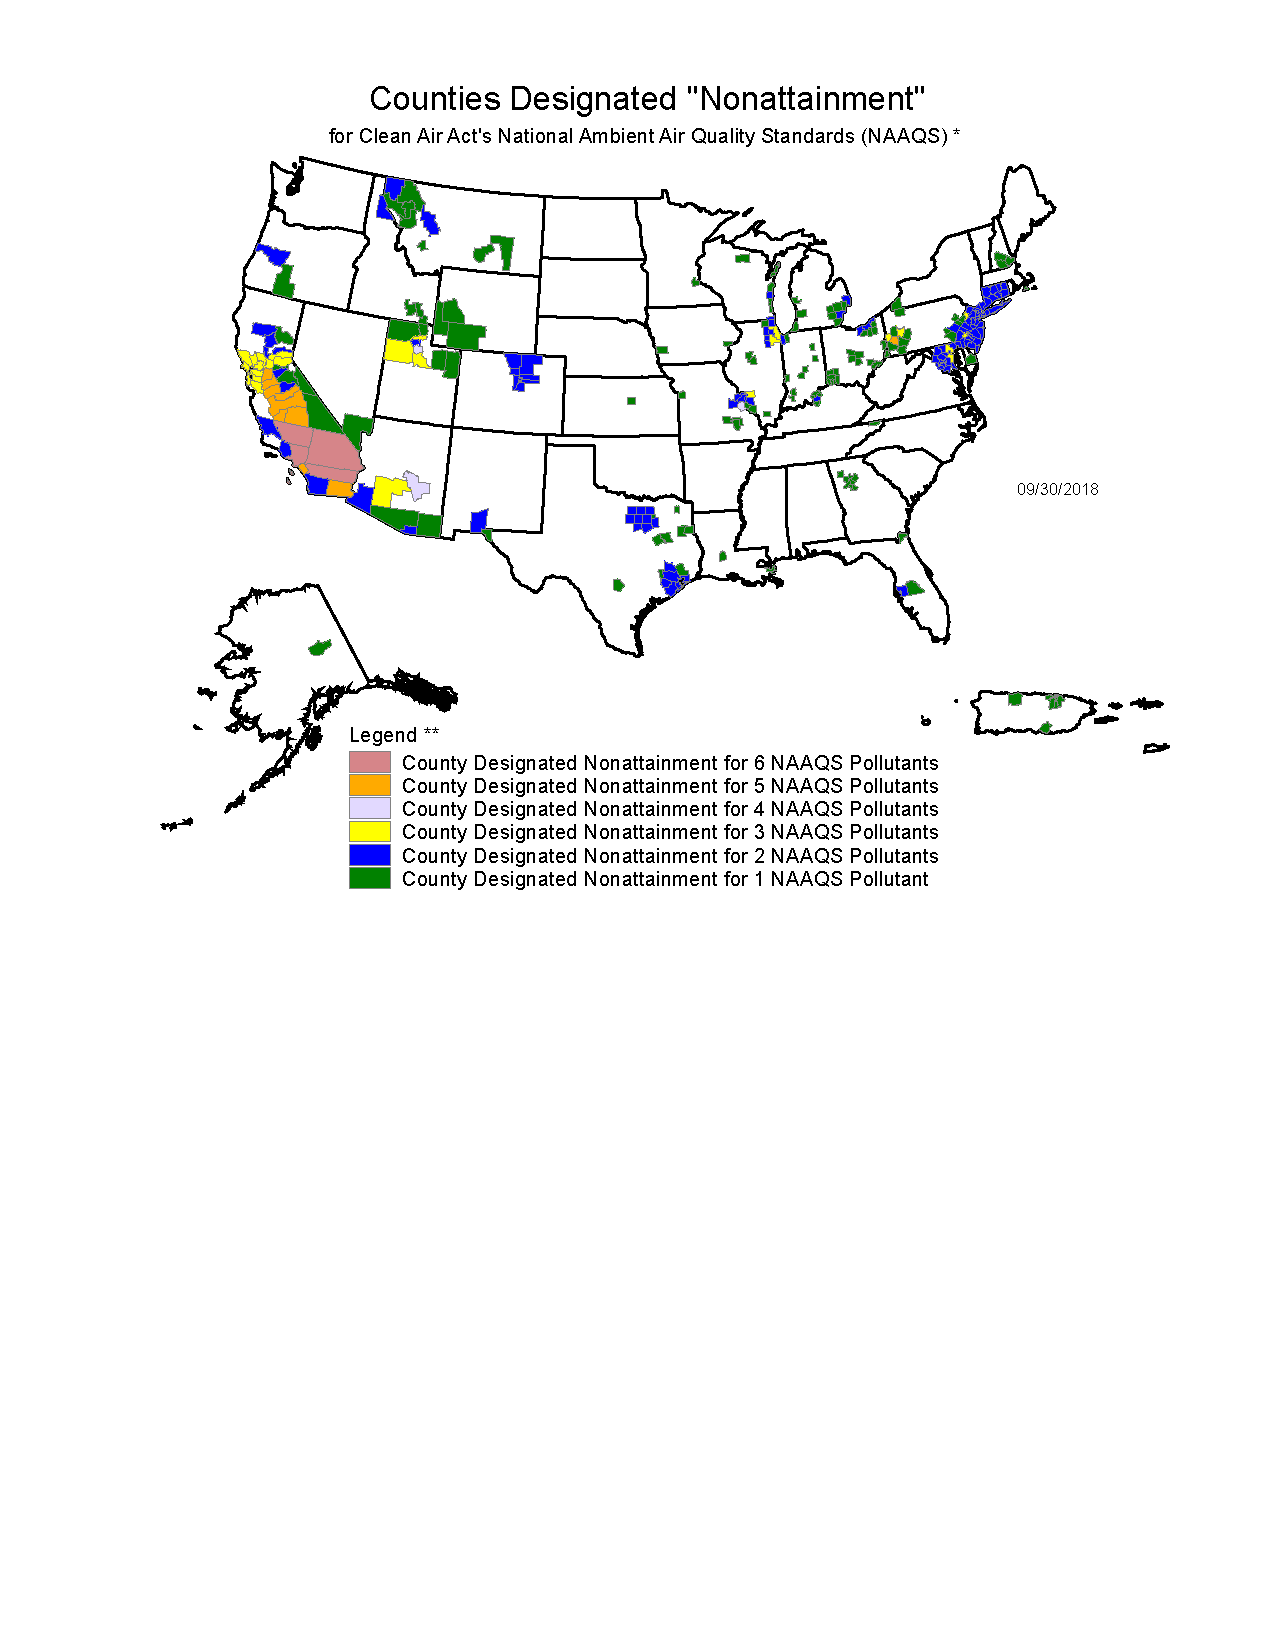
\includegraphics[width=\textwidth]{EPA_map_nonattain}
\caption*{}
\end{figure}
\end{columns}
\end{frame}


\begin{frame}{Why not linear regression?}

\begin{columns}
\column{0.4\textwidth}
For example:  EPA Criteria Pollutants.  For each region $i$ indicate nonattainment as follows:
\begin{itemize}
\item $y_i = 1 \rightarrow$ Ozone 
\item $y_i = 2 \rightarrow$ PM2.5 
\item $y_i = 3 \rightarrow$ PM10 
\item $y_i = 4 \rightarrow$ Sulfur Dioxide 
\item $y_i = 5 \rightarrow$ Lead 
\item $y_i = 6 \rightarrow$ Carbon Monoxide 
\item $y_i =7 \rightarrow$ Nitrogen Dioxide 
\end{itemize}

\column{0.55\textwidth}
Then,
\begin{align*}
y_i &= \beta\mathbf{x}_i + \epsilon
\end{align*}
where $\mathbf{x}_i$ is a vector of observed independent variables for each location $i$

\pause

\vspace{5mm}

The problem: a different ordering of variables would imply a different relationship between statuses, different models, and different predictions.
\end{columns}

\end{frame}

\begin{frame}{Predicting categorical variables the right way: Similar coding to using them as predictors}

\begin{columns}
\column{0.5\textwidth}
For example:  EPA Criteria Pollutants:
\begin{itemize}
\item $y_{i,1} \rightarrow$ Ozone status
\item $y_{i,2} \rightarrow$ PM2.5 status
\item $y_{i,3} \rightarrow$ PM10 status
\item $y_{i,4} \rightarrow$ Sulfur Dioxide status
\item $y_{i,5} \rightarrow$ Lead status
\item $y_{i,6} \rightarrow$ Carbon Monoxide status
\item $y_{i,7} \rightarrow$ Nitrogen Dioxide status
\end{itemize}
where $i$ indexes the region of interest, i.e. observations

\column{0.5\textwidth}
Then, for each, 
\begin{align*}
y_{i,j} &=\begin{cases}
    1, & \text{Nonattainment status}\\
    0, & \text{Attainment status}
  \end{cases}
\end{align*}
where $j$ indexes criteria pollutants
\end{columns}

\end{frame}

\begin{frame}{How do you get a model to output a $\{0,1\}$ result?}

\pause
\vspace{5mm}

\textbf{First,} build your model so that its output estimates a \textit{probability} that a given outcome happens.

\vspace{5mm}

For example, a model might give:

\vspace{5mm}
$p(\text{PM-2.5 nonattainment}) = 0.734$ and 
$p(\text{PM-2.5 attainment}) = 0.266$ 

\vspace{5mm}
(the probabilities add to one).

\end{frame}

\begin{frame}{How do you get a model to output a $\{0,1\}$ result? (ctd)}

\textbf{Second,} we use something called the \textit{Bayes Classifier}.  

\vspace{5mm}


\begin{block}{Bayes classifier:}
\textbf{} For a given observation $x_i$, choose $j$ as the value for which
\begin{align*}
\text{Pr}(Y=j|X = x_i)
\end{align*}
is largest. 
\end{block}

\vspace{5mm}

More formally,

\pause
\begin{align*}
\hat{y}_i = \arg \max_{j\in \mathcal{J}} \text{Pr}(Y=j|X = x_i)
\end{align*}
where $\mathcal{J}$ is the set of possible (mutually exclusive) outcomes.

\end{frame}

\begin{frame}{Classification error rate}

\textbf{If }the ``true model'' for $\Pr(Y=j|X = x_i)$ is known, then using the Bayes classifier will provide the lowest possible error rate.  

\vspace{5mm}

The \textit{error rate} quantifies how frequently a model mis-classifies a categorical variable.  

\vspace{5mm}
Let $I(\cdot)$ denote the \textit{indicator function}:

\pause
\begin{align*}
I(y_i \neq \hat{y}_i) &=\begin{cases}
    1, & \text{when } y_i \neq \hat{y}_i.\\
    0, & \text{otherwise}.
  \end{cases}  
  \end{align*}

\begin{align*}
\Rightarrow \text{error rate} = \frac{1}{n}\sum_{i=1}^n I (y_i \neq \hat{y}_i)
\end{align*}

\end{frame}

\begin{frame}{What's the error rate?}

\vspace{-8mm}

\begin{small}
\only<1>{\begin{table}[]
\begin{tabular}{lllll}
 &                   \textbf{Location}                       & \textbf{Actual status } & \textbf{Predicted  (hypothetical)}    & $I (y_i \neq \hat{y}_i)$ \\
 & Allegheny County, PA                  & Non-attainment & Non-attainment &                         \\
 & Cleveland, OH                         & Non-attainment & Non-attainment &                        \\
 & Delaware County, PA                   & Non-attainment & Non-attainment &                         \\
 & Imperial County, CA                   & Non-attainment & Attainment     &                         \\
 & Lebanon County, PA                    & Non-attainment & Attainment     &                         \\
 &South Coast Air Basin, CA & Non-attainment & Non-attainment &                         \\
 & Plumas County, CA                     & Non-attainment & Non-attainment &                         \\
 & Sacramento County, CA                 & Attainment     & Non-attainment &                        \\
 & San Francisco, CA                     & Attainment     & Non-attainment &                         \\
 & San Joaquin Valley, CA                & Non-attainment & Non-attainment &                         \\
 & West Silver Valley, ID                & Non-attainment & Non-attainment &                         \\
 & Luzerne County, PA                    & Attainment     & Attainment     &                        \\
 & Lancaster County, PA                  & Attainment     & Attainment     &                        
\end{tabular}
\end{table}}


\only<2>{\begin{table}[]
\begin{tabular}{lllll}
 &                               \textbf{Location}        & \textbf{Actual status } & \textbf{Predicted  (hypothetical)}    & $I (y_i \neq \hat{y}_i)$ \\
 & Allegheny County, PA                  & Non-attainment & Non-attainment & 0                        \\
 & Cleveland, OH                         & Non-attainment & Non-attainment & 0                        \\
 & Delaware County, PA                   & Non-attainment & Non-attainment & 0                        \\
 & Imperial County, CA                   & Non-attainment & Attainment     &                        \\
 & Lebanon County, PA                    & Non-attainment & Attainment     &                        \\
 &South Coast Air Basin, CA & Non-attainment & Non-attainment &                   \\
 & Plumas County, CA                     & Non-attainment & Non-attainment &                         \\
 & Sacramento County, CA                 & Attainment     & Non-attainment &                        \\
 & San Francisco, CA                     & Attainment     & Non-attainment &                        \\
 & San Joaquin Valley, CA                & Non-attainment & Non-attainment &                        \\
 & West Silver Valley, ID                & Non-attainment & Non-attainment &                     \\
 & Luzerne County, PA                    & Attainment     & Attainment     &             \\
 & Lancaster County, PA                  & Attainment     & Attainment     &              
\end{tabular}
\end{table}}



\only<3>{\begin{table}[]
\begin{tabular}{lllll}
 &                               \textbf{Location}        & \textbf{Actual status } & \textbf{Predicted  (hypothetical)}    & $I (y_i \neq \hat{y}_i)$ \\
 & Allegheny County, PA                  & Non-attainment & Non-attainment & 0                        \\
 & Cleveland, OH                         & Non-attainment & Non-attainment & 0                        \\
 & Delaware County, PA                   & Non-attainment & Non-attainment & 0                        \\
 & Imperial County, CA                   & Non-attainment & Attainment     & 1                        \\
 & Lebanon County, PA                    & Non-attainment & Attainment     & 1                        \\
 &South Coast Air Basin, CA & Non-attainment & Non-attainment & 0                        \\
 & Plumas County, CA                     & Non-attainment & Non-attainment & 0                        \\
 & Sacramento County, CA                 & Attainment     & Non-attainment &                         \\
 & San Francisco, CA                     & Attainment     & Non-attainment &                         \\
 & San Joaquin Valley, CA                & Non-attainment & Non-attainment &                         \\
 & West Silver Valley, ID                & Non-attainment & Non-attainment &                         \\
 & Luzerne County, PA                    & Attainment     & Attainment     &                        \\
 & Lancaster County, PA                  & Attainment     & Attainment     &                        
\end{tabular}
\end{table}}

\only<4>{\begin{table}[]
\begin{tabular}{lllll}
 &                               \textbf{Location}        & \textbf{Actual status } & \textbf{Predicted  (hypothetical)}    & $I (y_i \neq \hat{y}_i)$ \\
 & Allegheny County, PA                  & Non-attainment & Non-attainment & 0                        \\
 & Cleveland, OH                         & Non-attainment & Non-attainment & 0                        \\
 & Delaware County, PA                   & Non-attainment & Non-attainment & 0                        \\
 & Imperial County, CA                   & Non-attainment & Attainment     & 1                        \\
 & Lebanon County, PA                    & Non-attainment & Attainment     & 1                        \\
 &South Coast Air Basin, CA & Non-attainment & Non-attainment & 0                        \\
 & Plumas County, CA                     & Non-attainment & Non-attainment & 0                        \\
 & Sacramento County, CA                 & Attainment     & Non-attainment & 1                        \\
 & San Francisco, CA                     & Attainment     & Non-attainment & 1                        \\
 & San Joaquin Valley, CA                & Non-attainment & Non-attainment & 0                        \\
 & West Silver Valley, ID                & Non-attainment & Non-attainment & 0                        \\
 & Luzerne County, PA                    & Attainment     & Attainment     & 0                       \\
 & Lancaster County, PA                  & Attainment     & Attainment     & 0                       
\end{tabular}
\end{table}}

\pause\pause\pause
\end{small}

\begin{center}
$\rightarrow$ Overall error rate is $\frac{1}{13}\cdot 4 = .31$
\end{center}
\end{frame}


\begin{frame}{Finally, the decision boundary}
\begin{columns}
\column{0.55\textwidth}
\begin{figure}
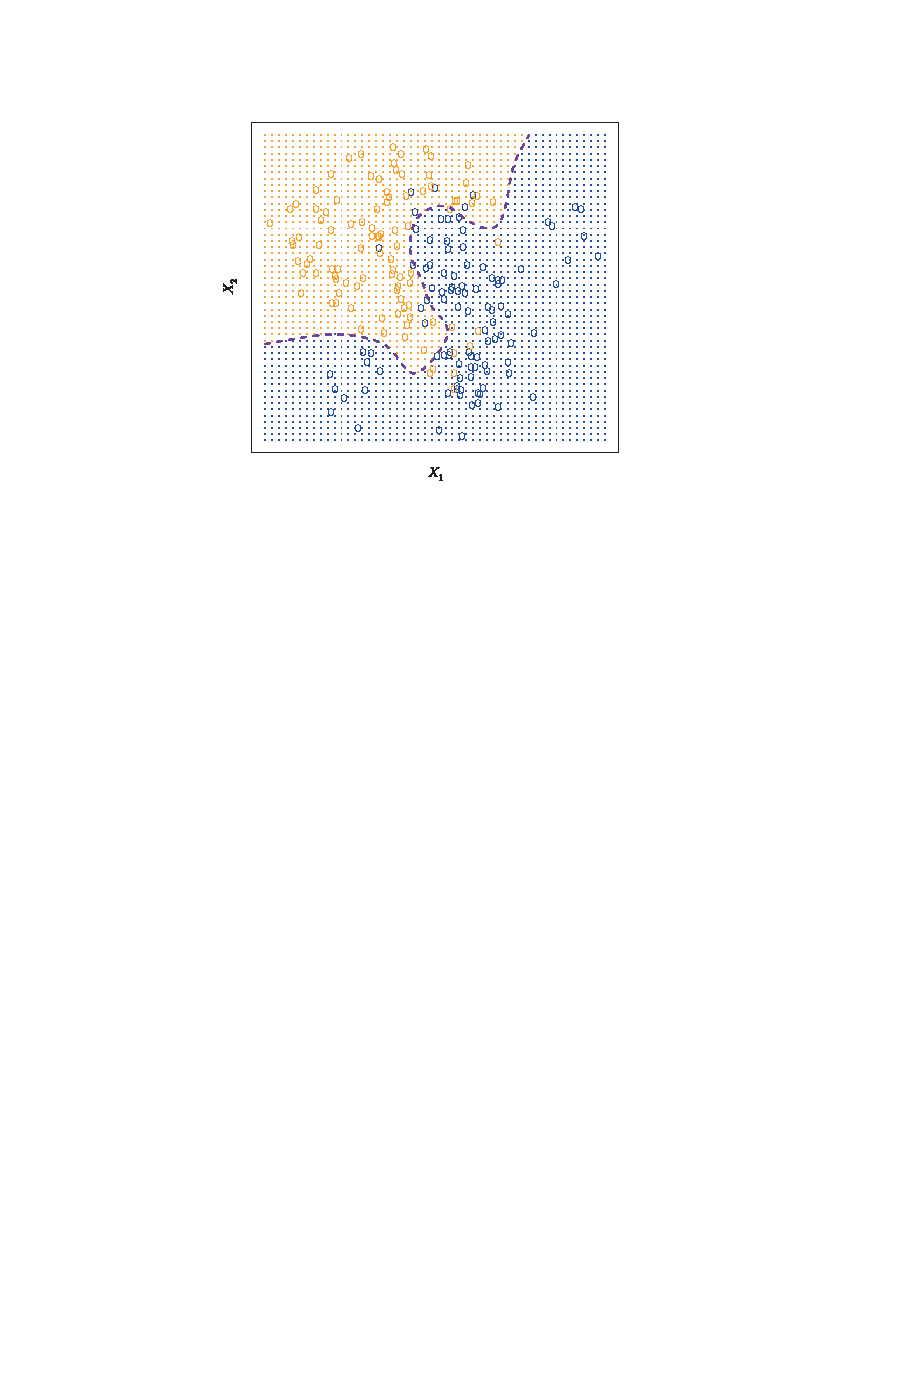
\includegraphics[width=\textwidth]{bayes_decision_boundary}
\caption*{ISLR Fig 2.13}
\end{figure}
\column{0.35\textwidth}
Along the boundary, what condition holds?  \pause \textbf{The probability of one outcome equals the probability of the other.}

\vspace{5mm}

If the true model  $\Pr(Y=j|X = x_i)$ is known, we call this the \textbf{Bayes decision boundary.}

\vspace{5mm}

All methods try to \textit{estimate} the Bayes decision boundary.  

\end{columns}
\end{frame}


\begin{frame}{KNN for categorical variables}

It's pretty simple!  Estimate the probabilities as


\uncover<2->{
$  $\begin{align*}
\Pr (Y=j|X=x_0) = \frac{1}{K} \sum_{i\in \mathcal{N}_0} I(y_i = j)
\end{align*}}

$K =$ number of neighboring \textbf{\textit{training}} points to consider

 $\mathcal{N}_0 = $ set of $K$ \textbf{\textit{training}} points closest to observation $x_0$.
 
 \vspace{5mm}
 
...Then apply the Bayes classifier to choose the outcome variable.

 
\uncover<2->{\begin{align*}
\hat{y}_i = \arg \max_{j\in \mathcal{J}} \text{Pr}(Y=j|X = x_i)
\end{align*}
where $x_i$ is any feasible point in the space of independent variables.}
\end{frame}

\begin{frame}{Simple KNN Example, $K = 3$}

\begin{figure}
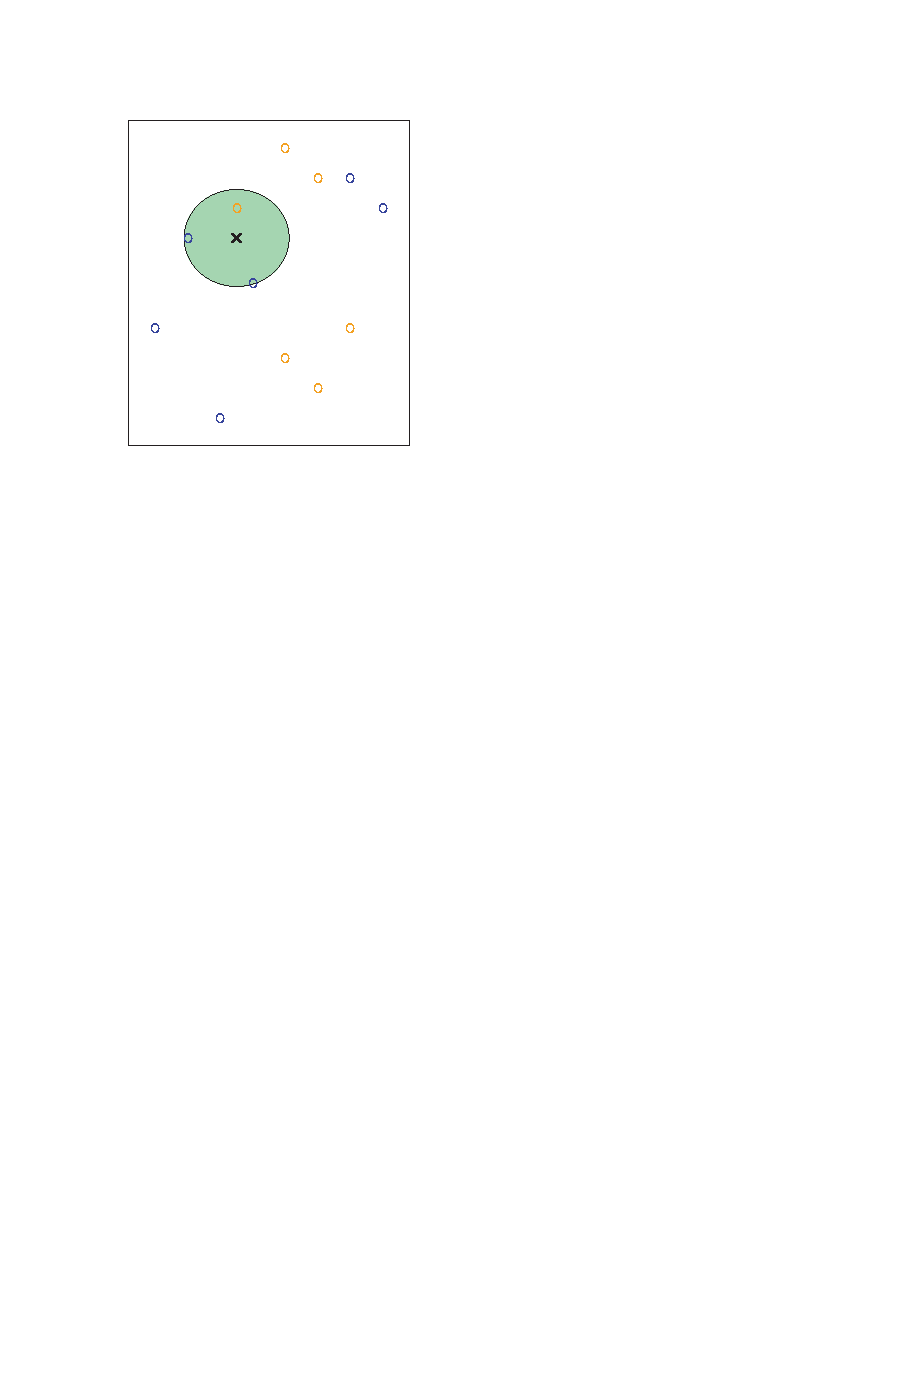
\includegraphics[width=0.4\textwidth]{KNN_example_1}
\pause 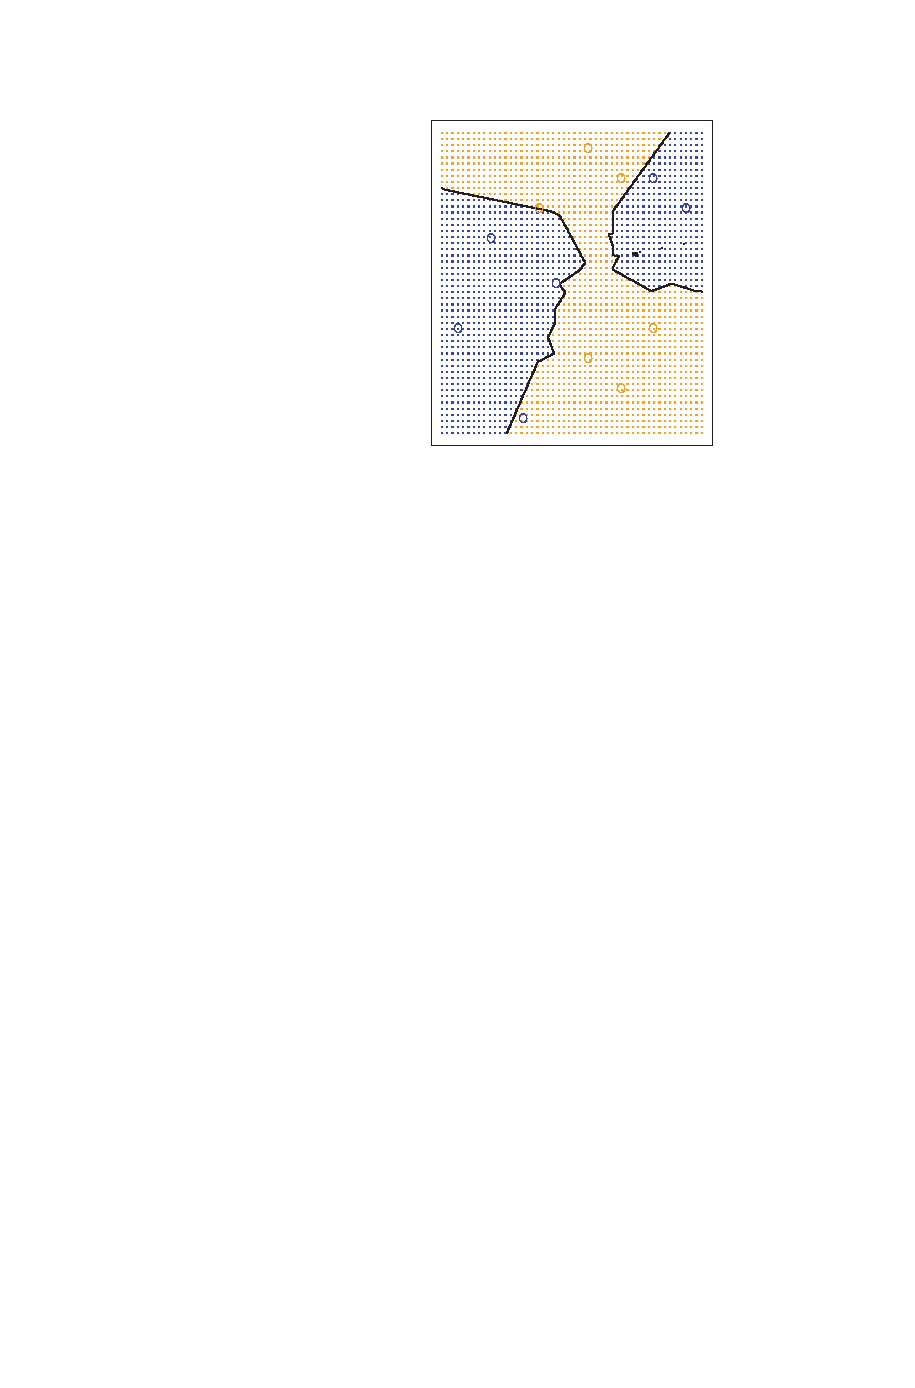
\includegraphics[width=0.4\textwidth]{KNN_example_2}
\caption*{ISLR Fig 2.14}
\end{figure}
\end{frame}

\begin{frame}{Which has the highest $K$?  Which has the lowest?}

\textbf{Dashed} = Bayes decision boundary

\textbf{Solid} = KNN estimate of Bayes decision boundary
\begin{columns}
\column{0.33\textwidth}
\begin{figure}
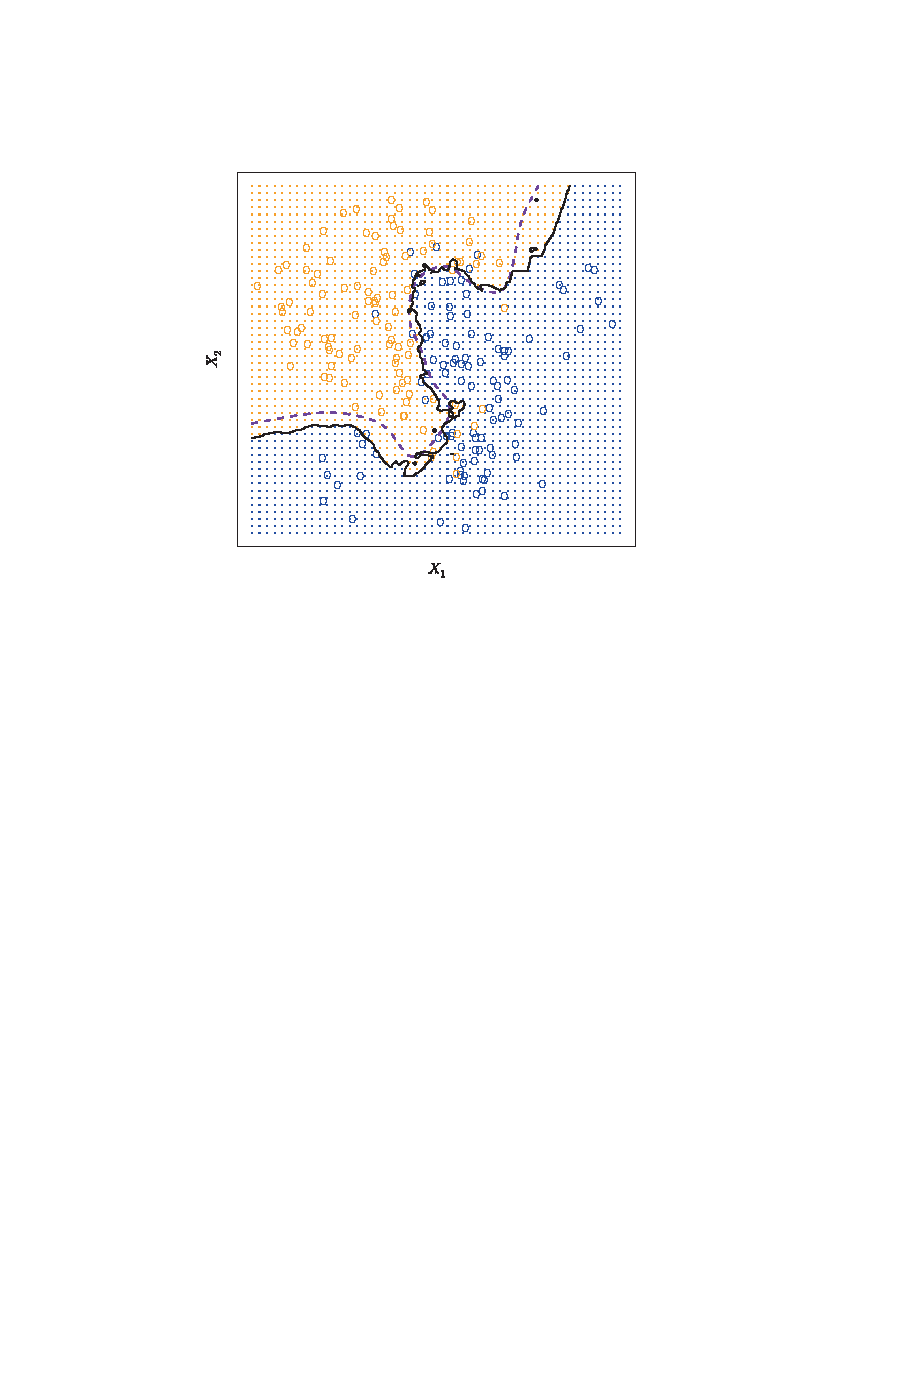
\includegraphics[width=\textwidth]{KNN_k10}
\caption*{\uncover<2->{K = 10}}
\end{figure}

\column{0.33\textwidth}
\begin{figure}
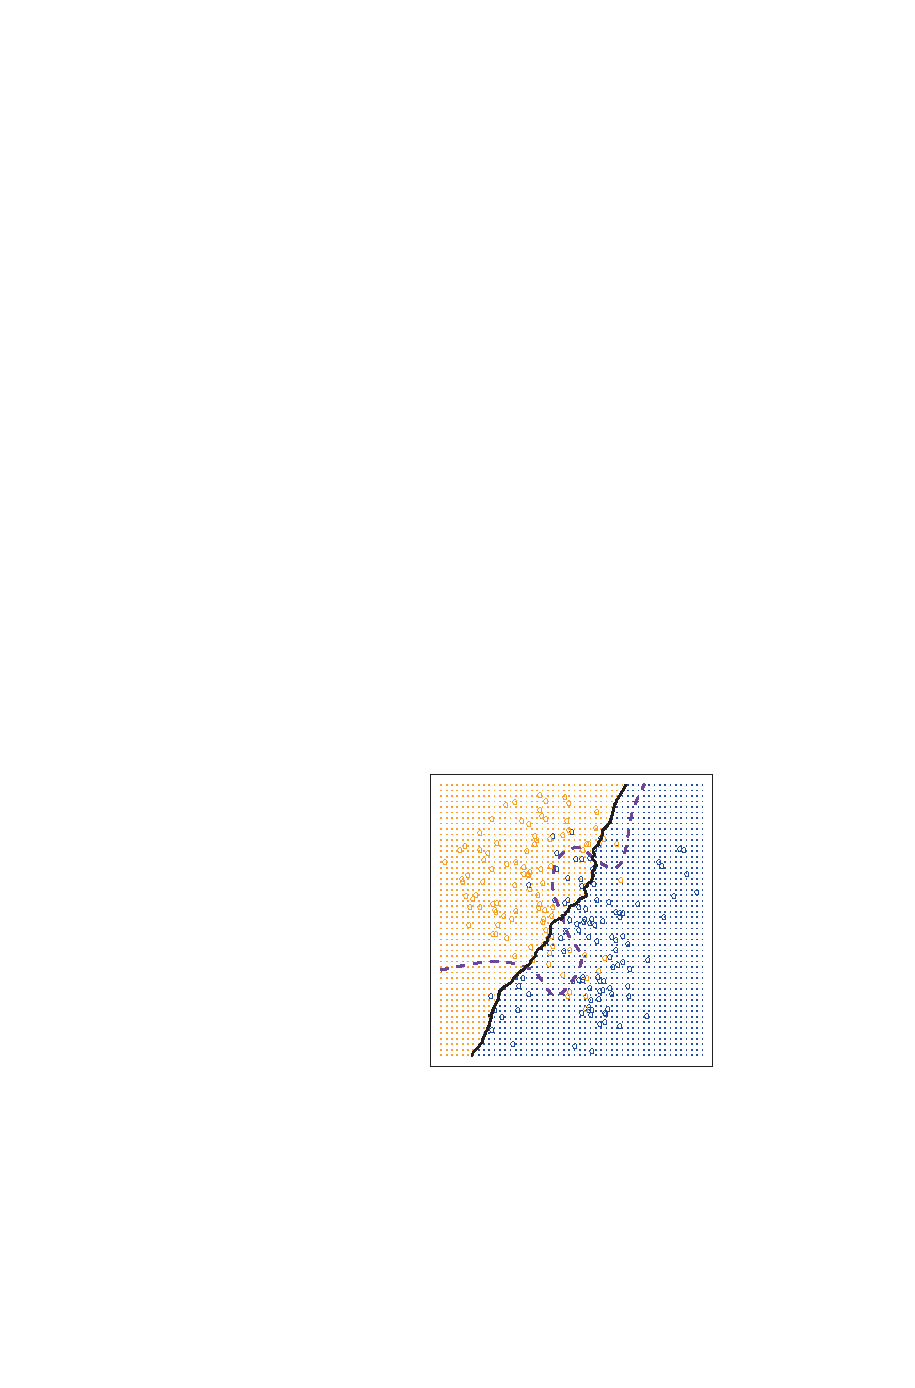
\includegraphics[width=\textwidth]{KNN_k100}
\caption*{\uncover<2->{K = 100}}
\end{figure}

\column{0.33\textwidth}
\begin{figure}
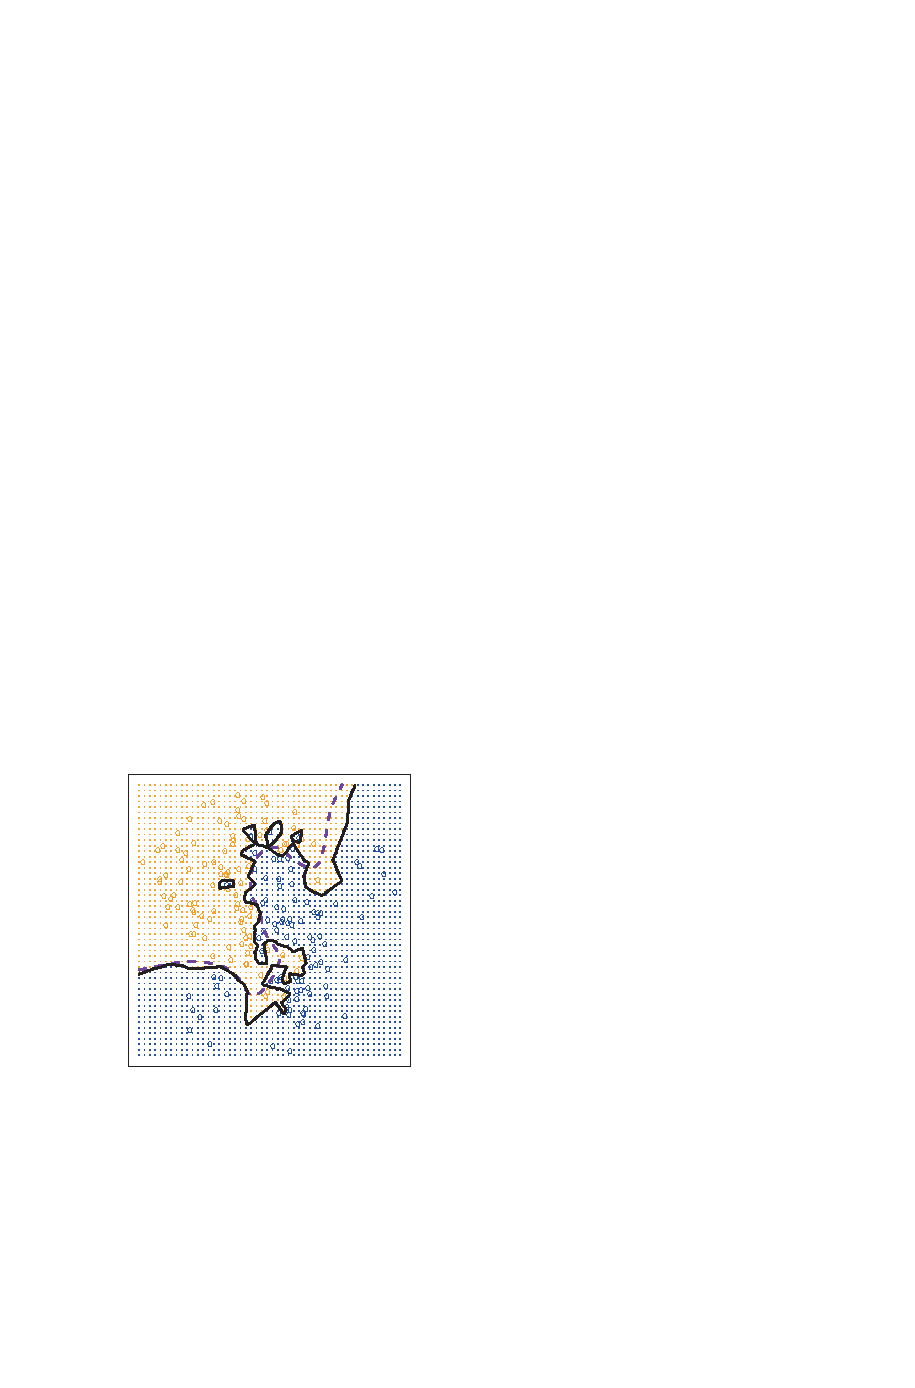
\includegraphics[width=\textwidth]{KNN_k1}
\caption*{\uncover<2->{K = 1}}
\end{figure}
\end{columns}
\end{frame}

\begin{frame}{KNN test and training error}

\only<1>{\begin{figure}
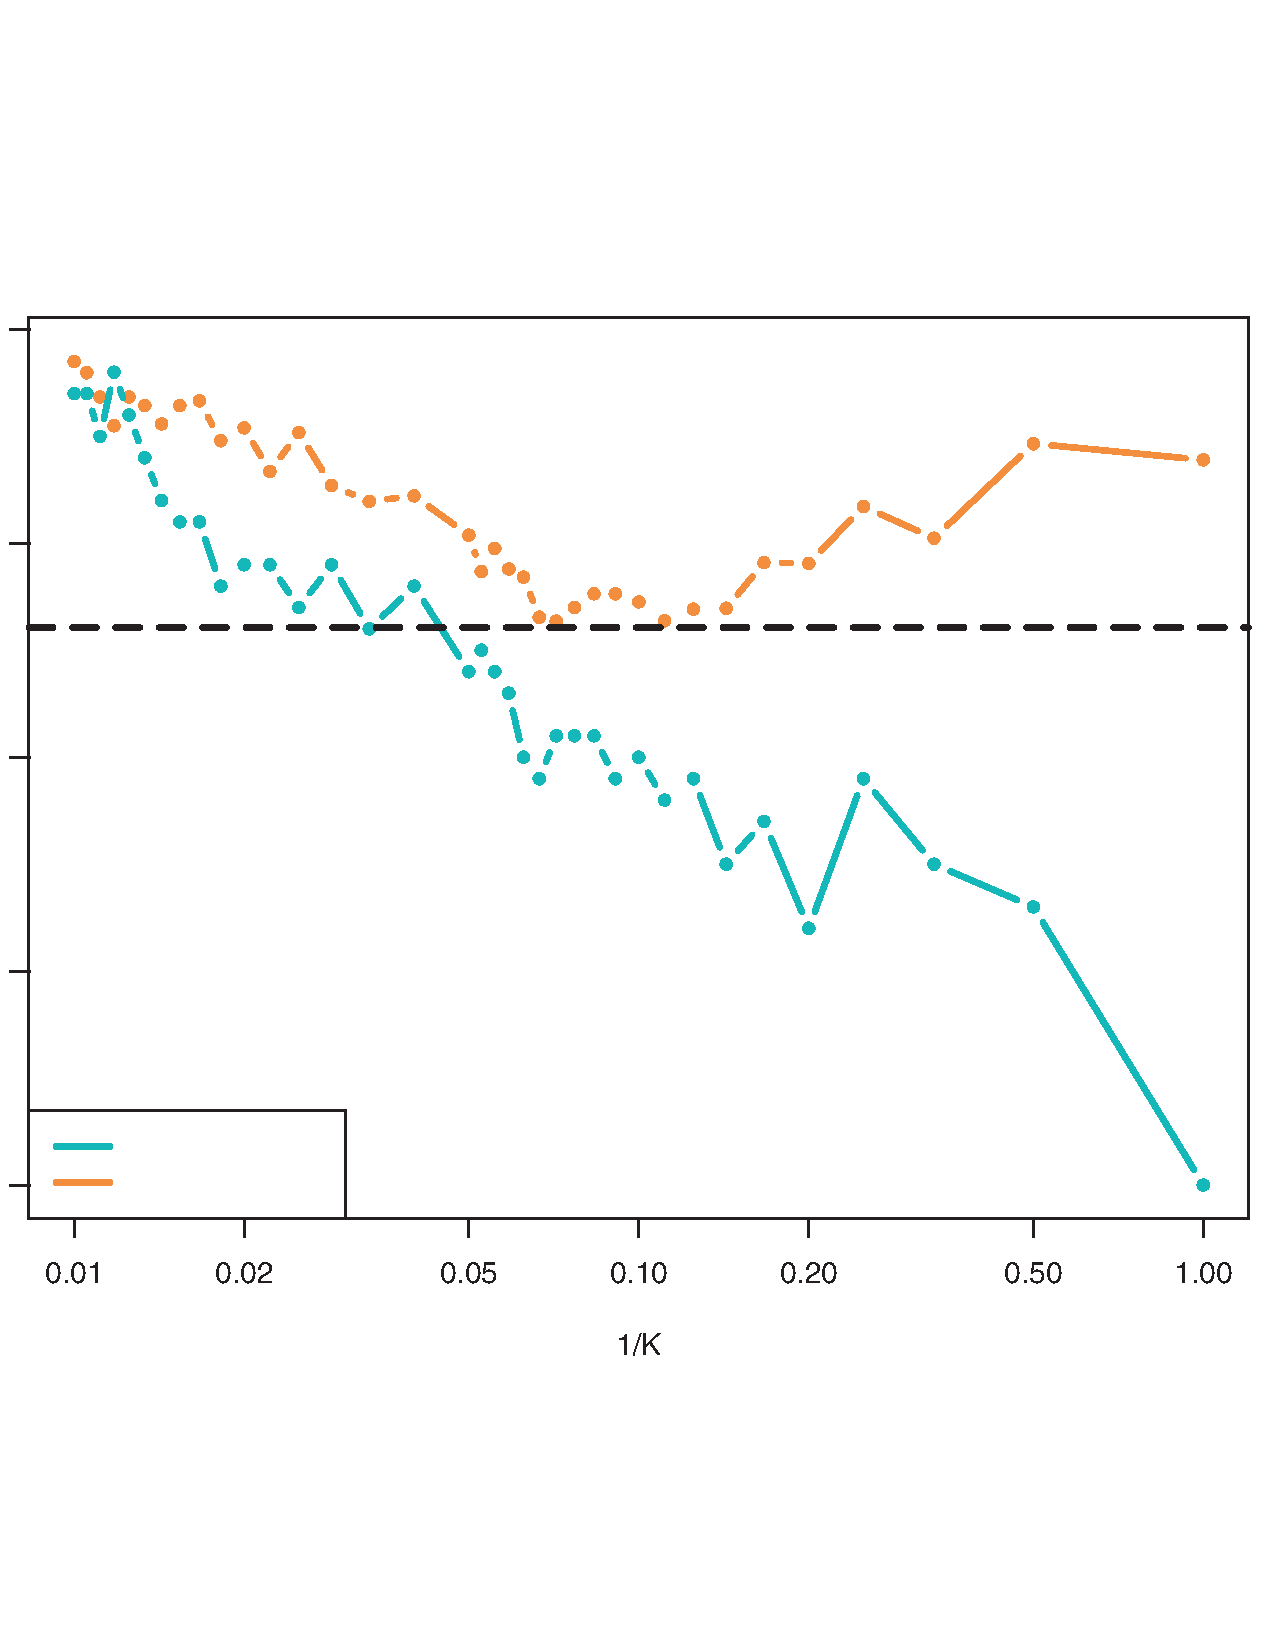
\includegraphics[height=0.8\textheight]{test_train_KNN_nolabel}
\caption*{ISLR 2.17}
\end{figure}}


\only<2>{\begin{figure}
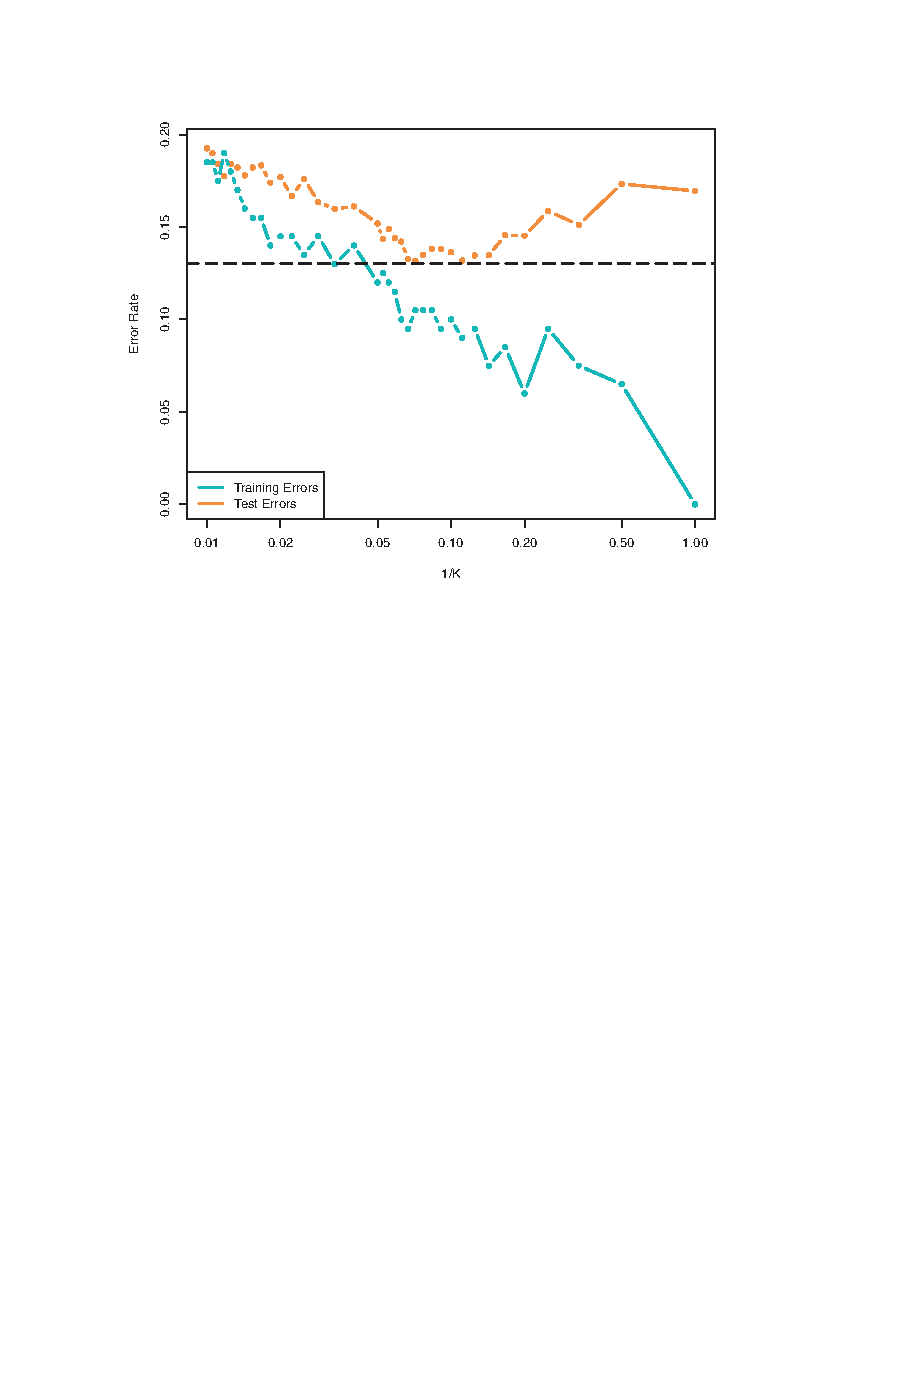
\includegraphics[height=0.8\textheight]{test_train_KNN_label}
\caption*{ISLR 2.17}
\end{figure}}

\end{frame}

\begin{frame}{How would KNN perform with nonattainment areas?}

\begin{columns}
\column{0.6\textwidth}
\begin{figure}
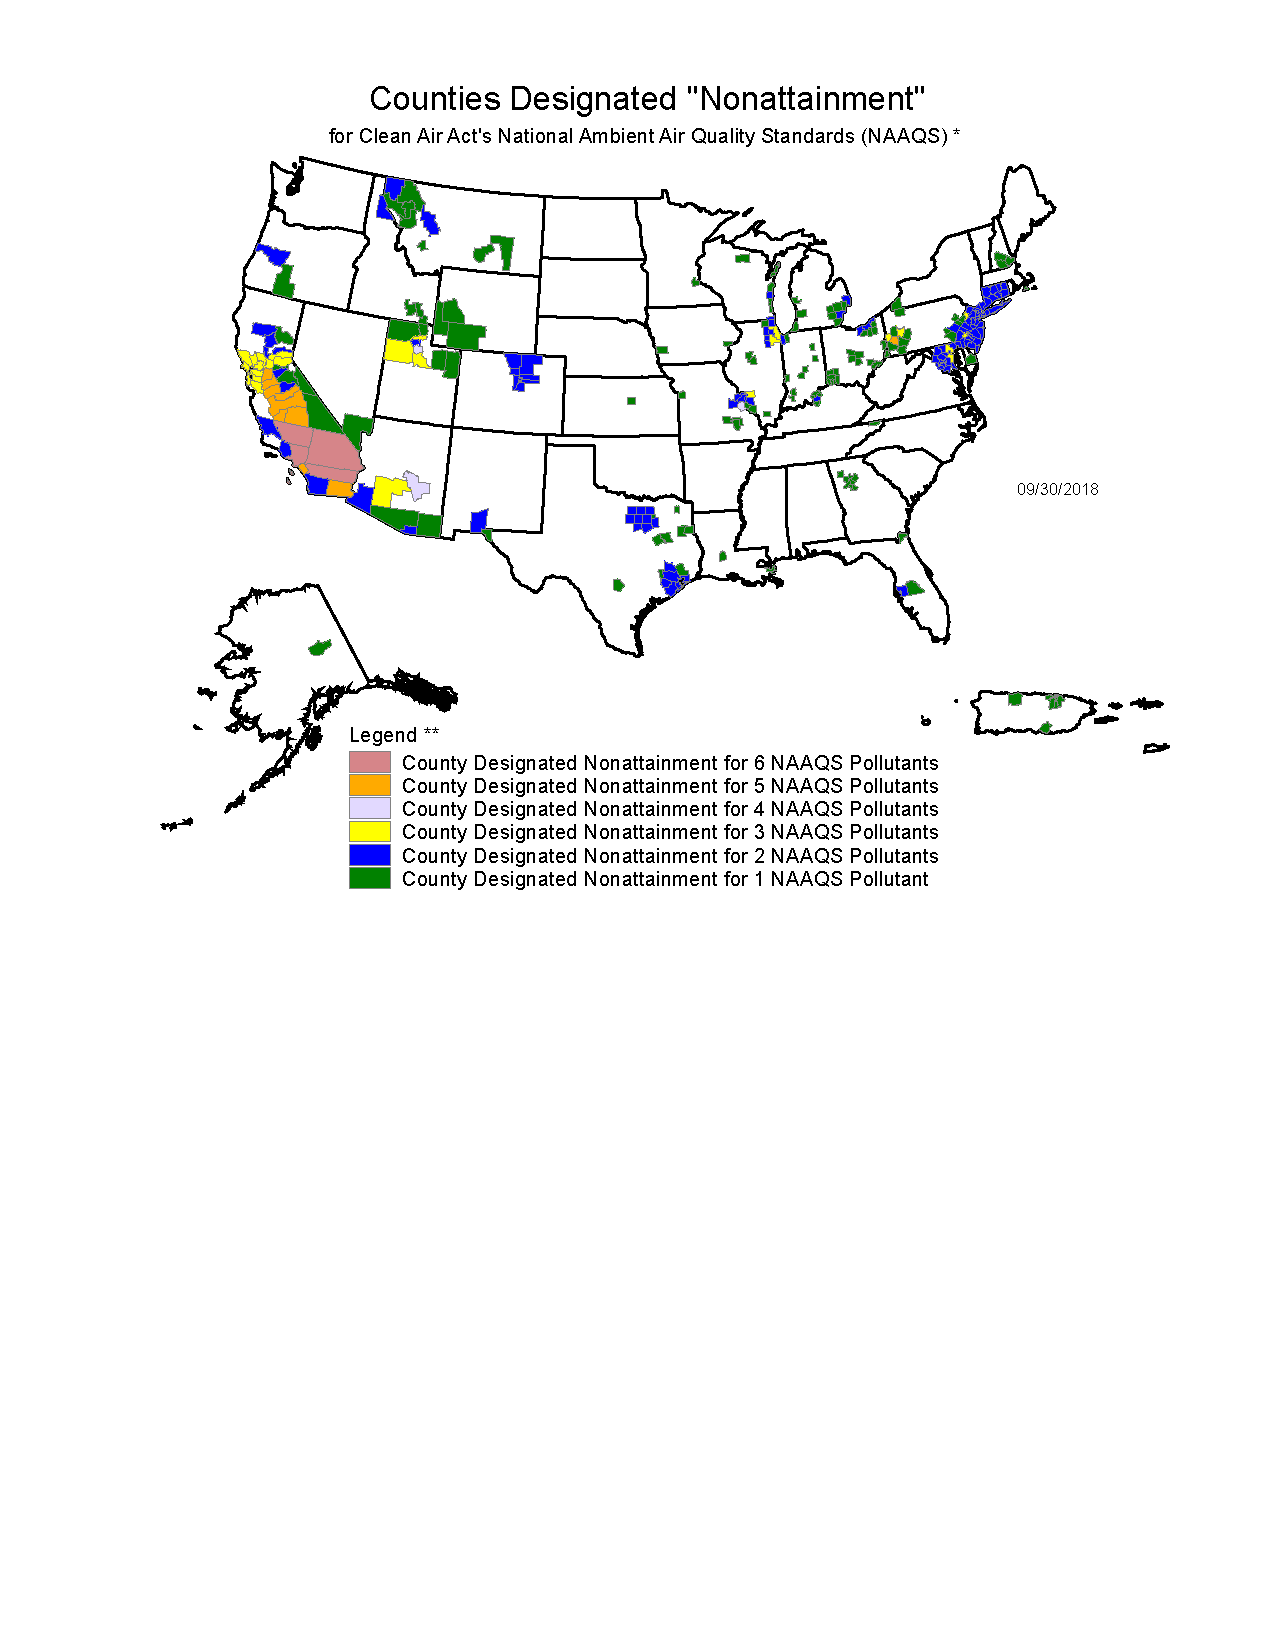
\includegraphics[width=\textwidth]{EPA_map_nonattain}
\caption*{}
\end{figure}
\column{0.4\textwidth}
\pause
\begin{itemize}
\item Challenge: If we only use location as independent variables, the Bayes decision boundary is very complex!
\item But if we use other independent variables (a simple one would be local emissions) we might do ok.
\end{itemize}
\end{columns}
\end{frame}

\begin{frame}{Clasification application example: Predicting water quality violations}

Seigi Karasaki, last year's ER131 GSI, has a work in progress to predict water quality violations in small community water systems in California.\\~\\
He kindly shared the next several slides with me.

\end{frame}


\begin{frame}
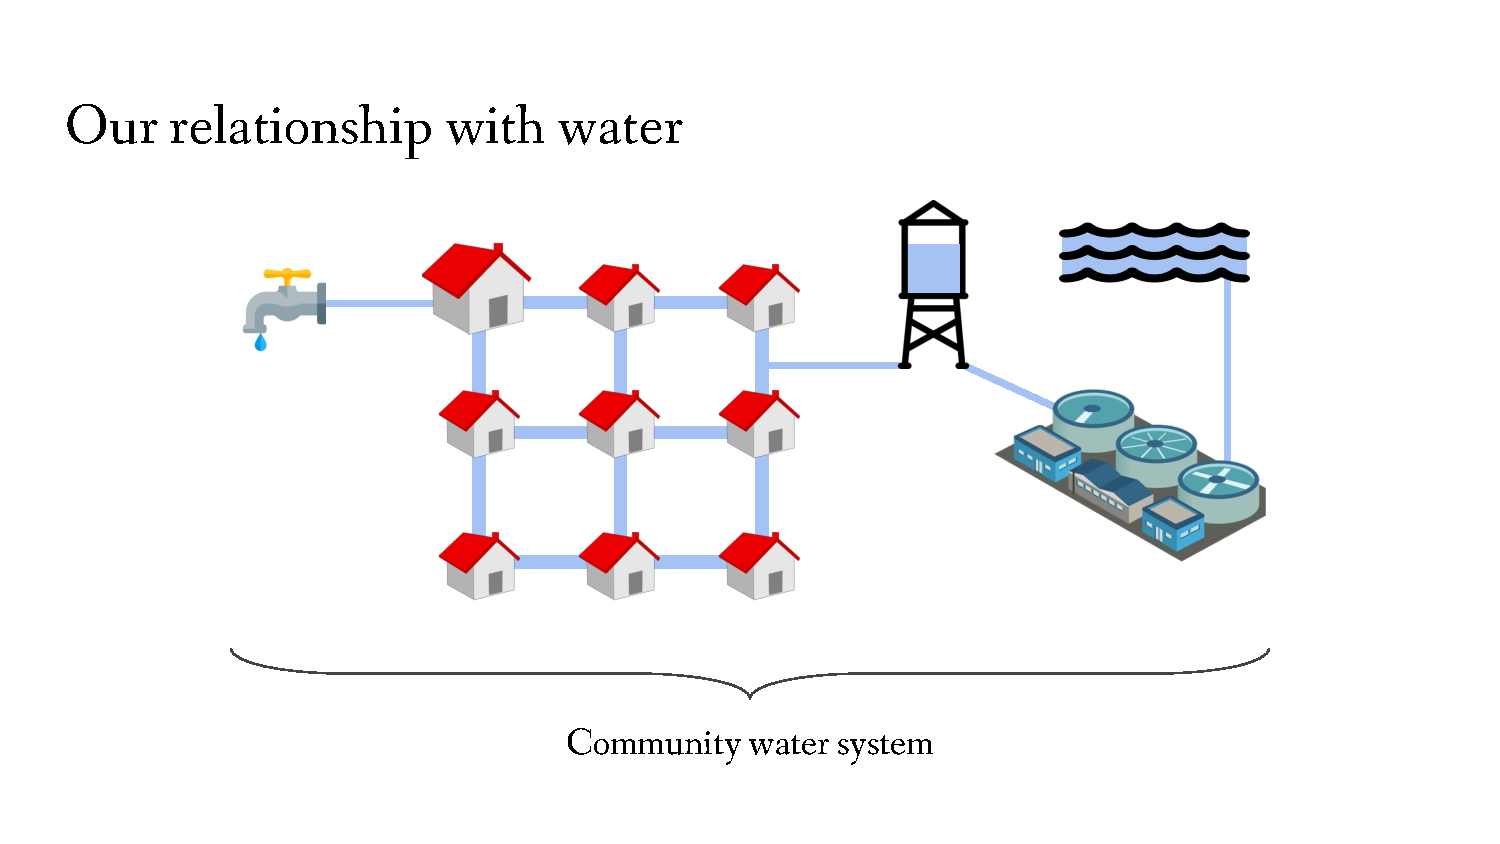
\includegraphics[width=1.2\textwidth]{seigi_2}
\end{frame}

\begin{frame}
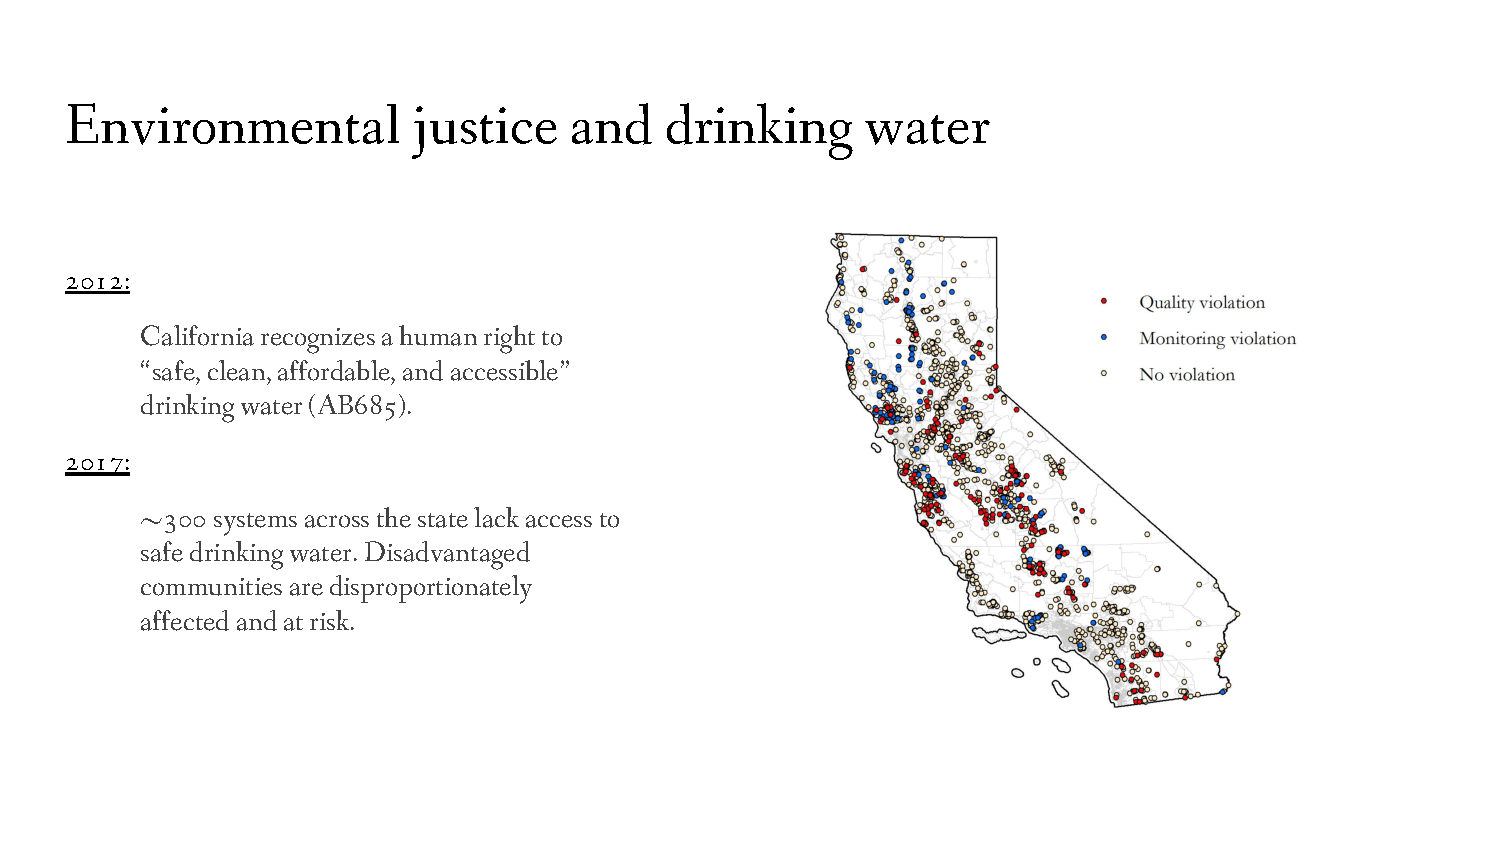
\includegraphics[width=1.2\textwidth]{seigi_1}
\end{frame}

\begin{frame}
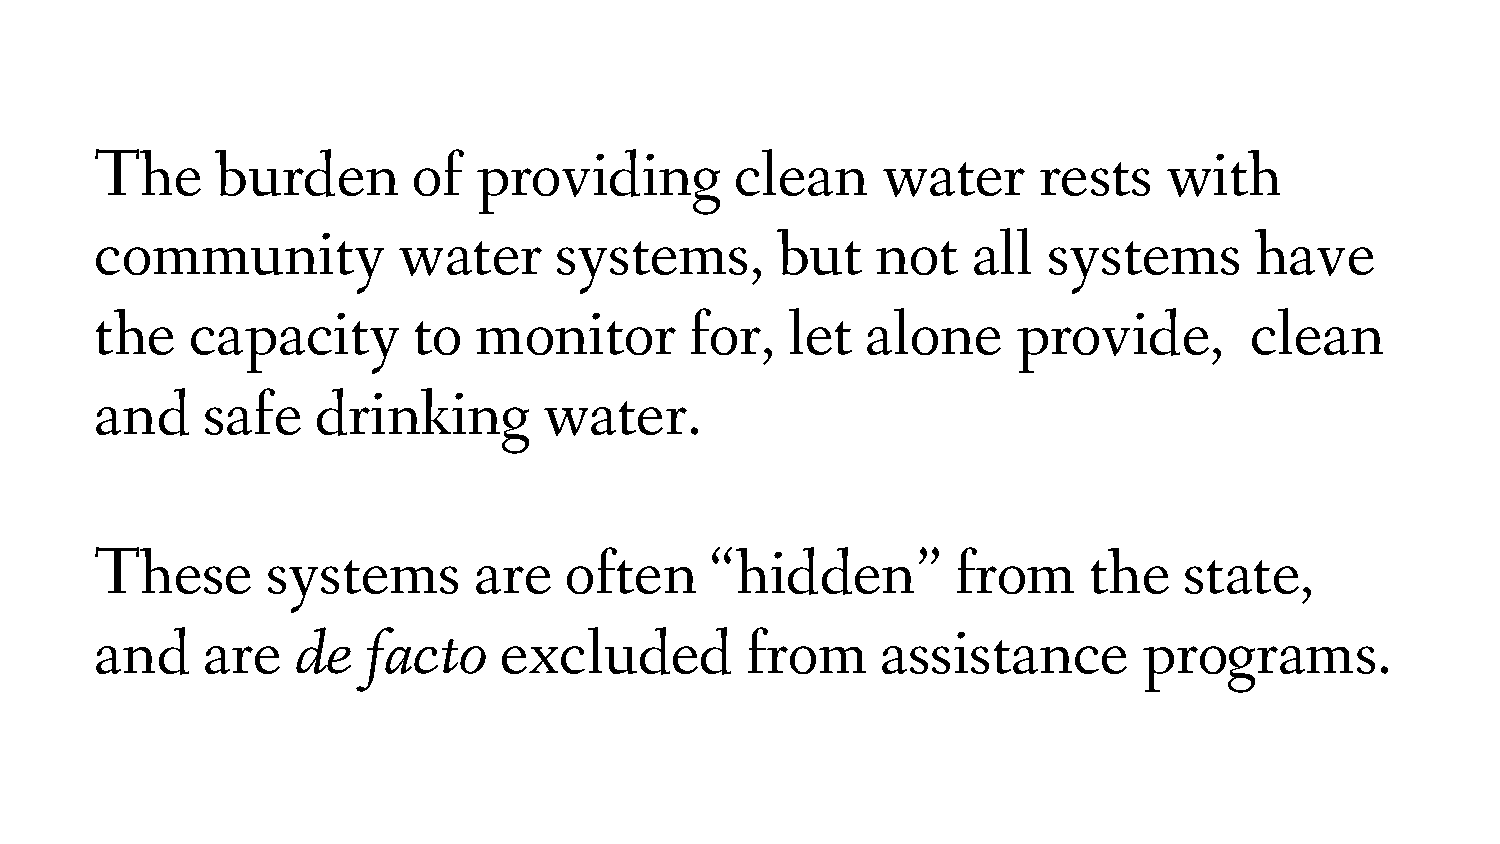
\includegraphics[width=1.1\textwidth]{seigi_3}
\end{frame}

\begin{frame}
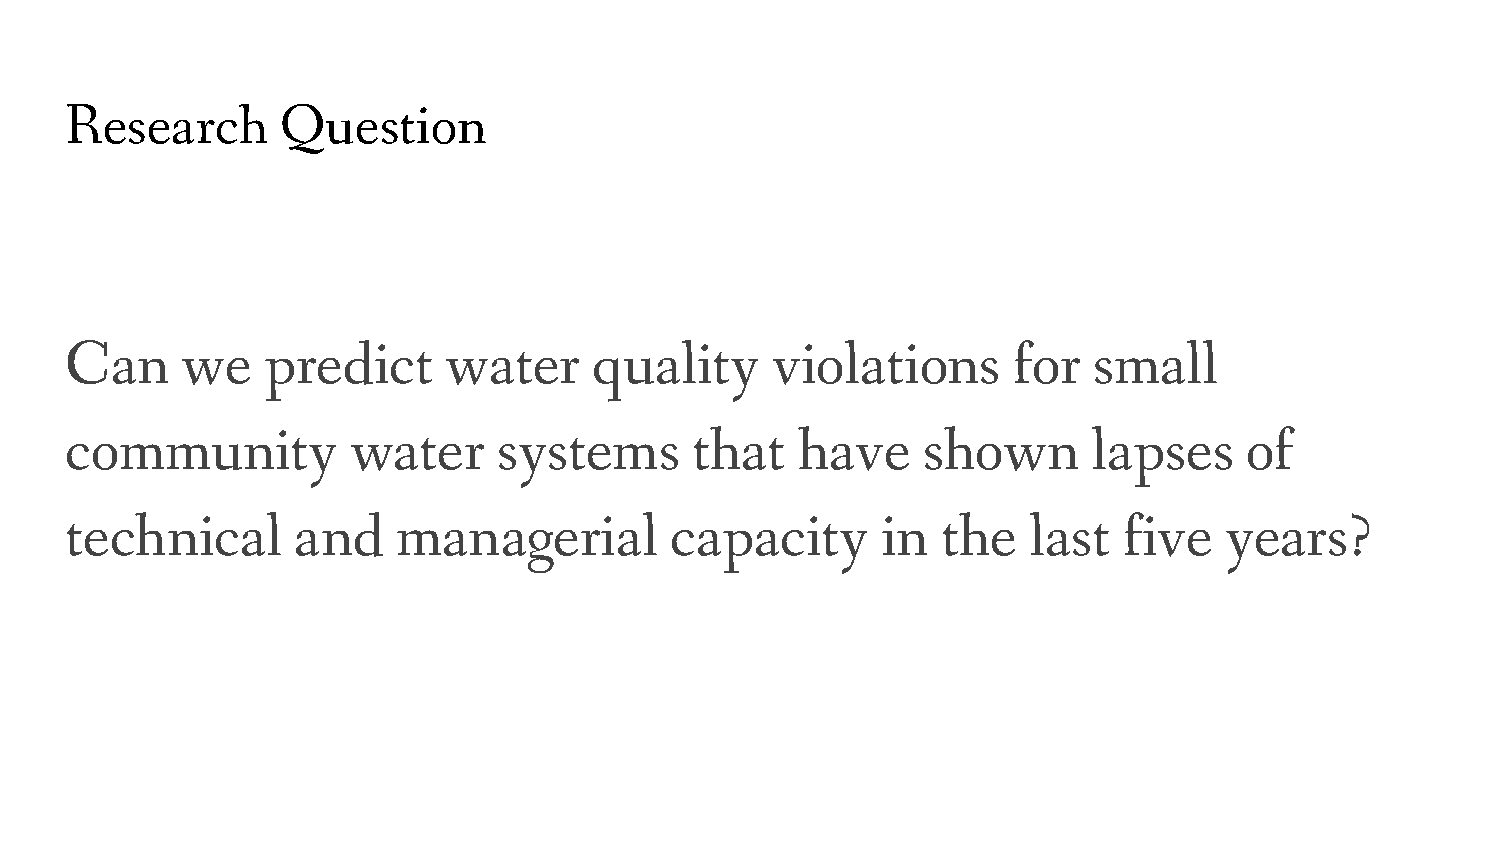
\includegraphics[width=1.1\textwidth]{seigi_5}
\end{frame}

\begin{frame}
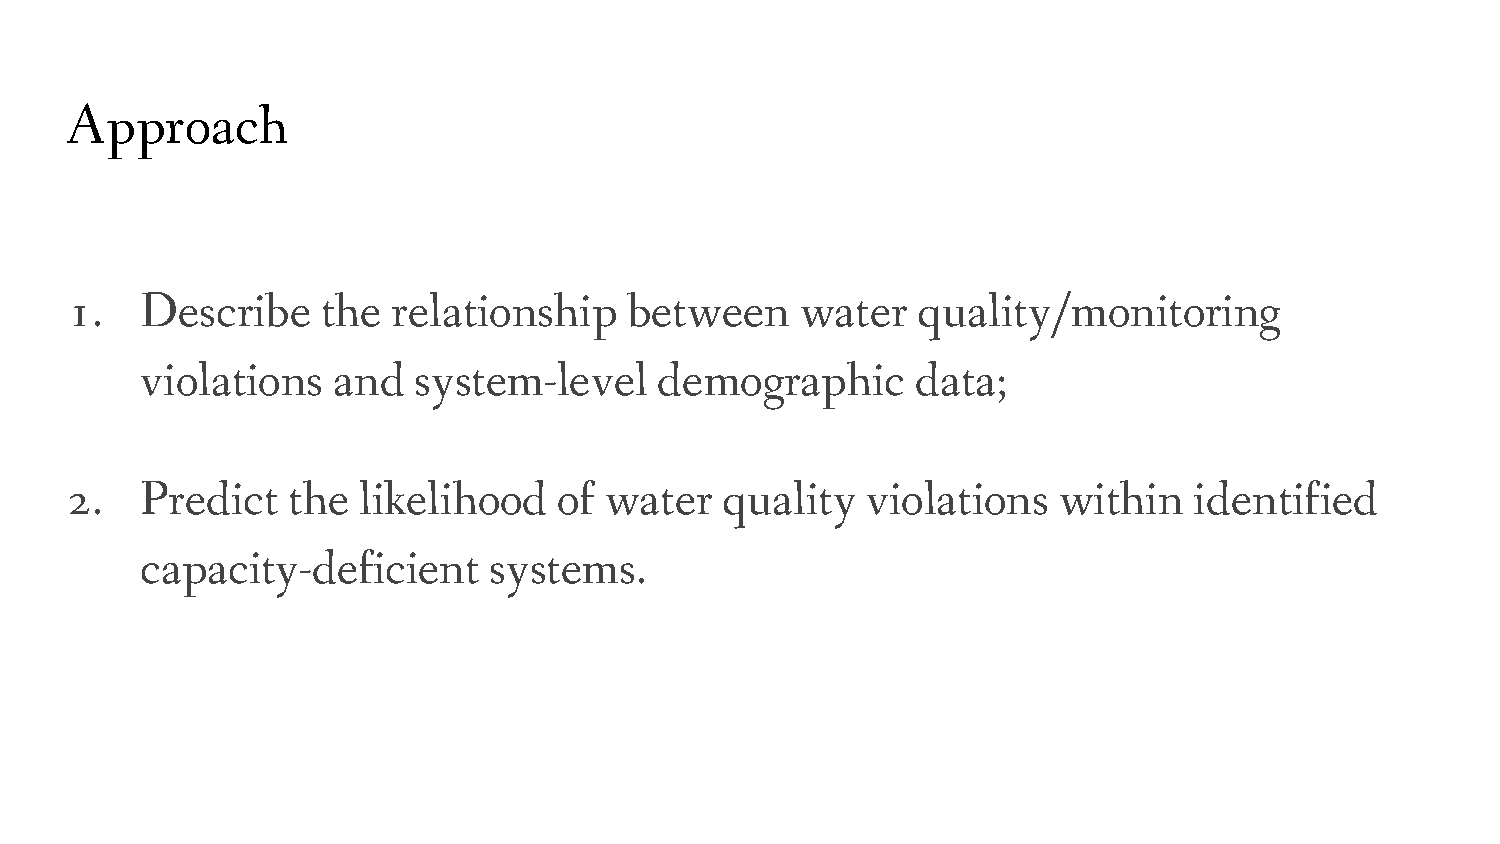
\includegraphics[width=1.1\textwidth]{seigi_6}
\end{frame}

\begin{frame}
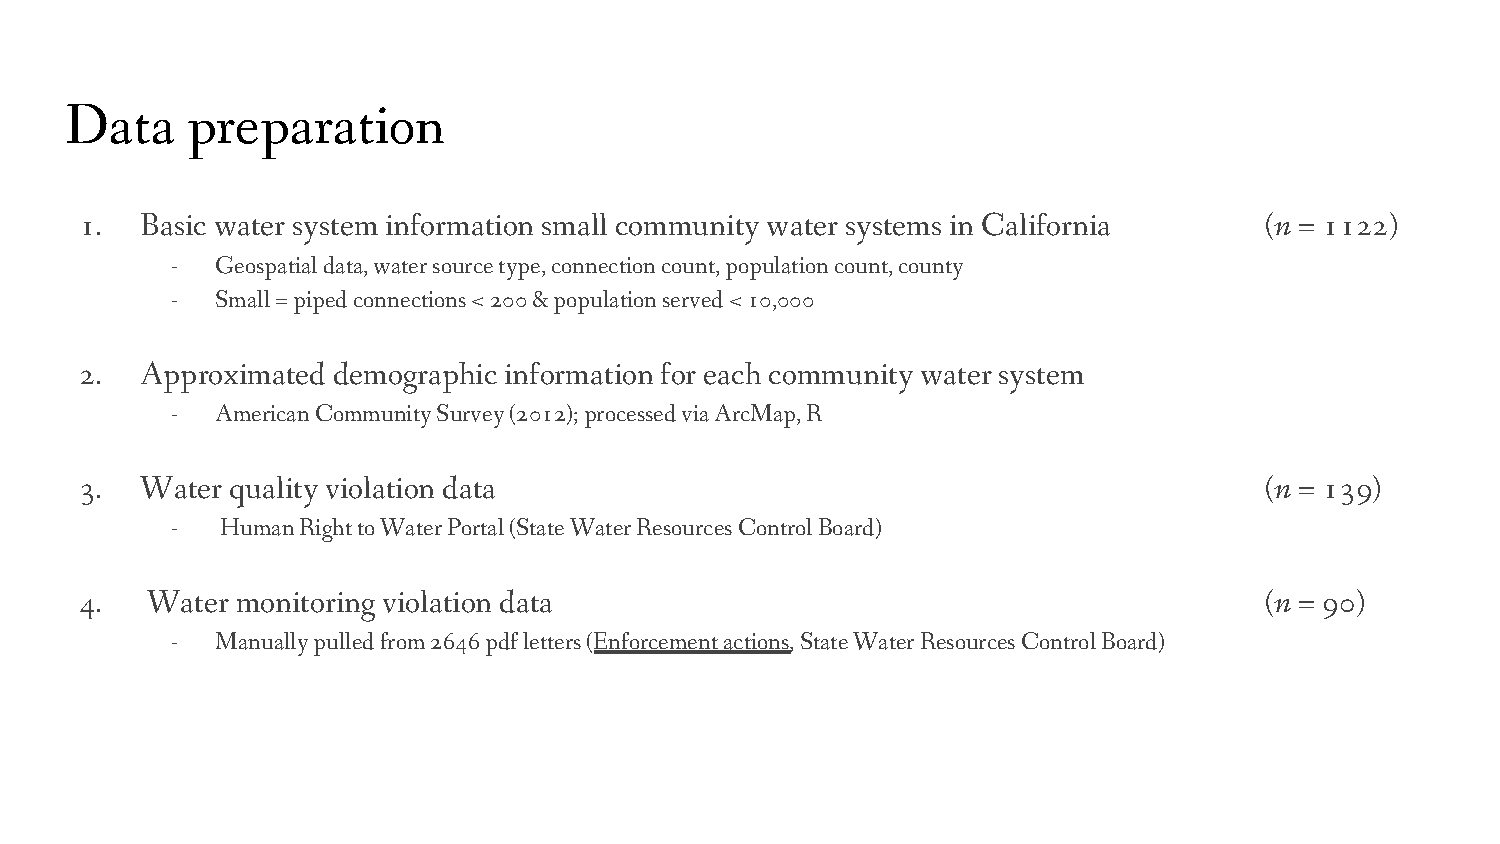
\includegraphics[width=1.1\textwidth]{seigi_7}
\end{frame}

\begin{frame}
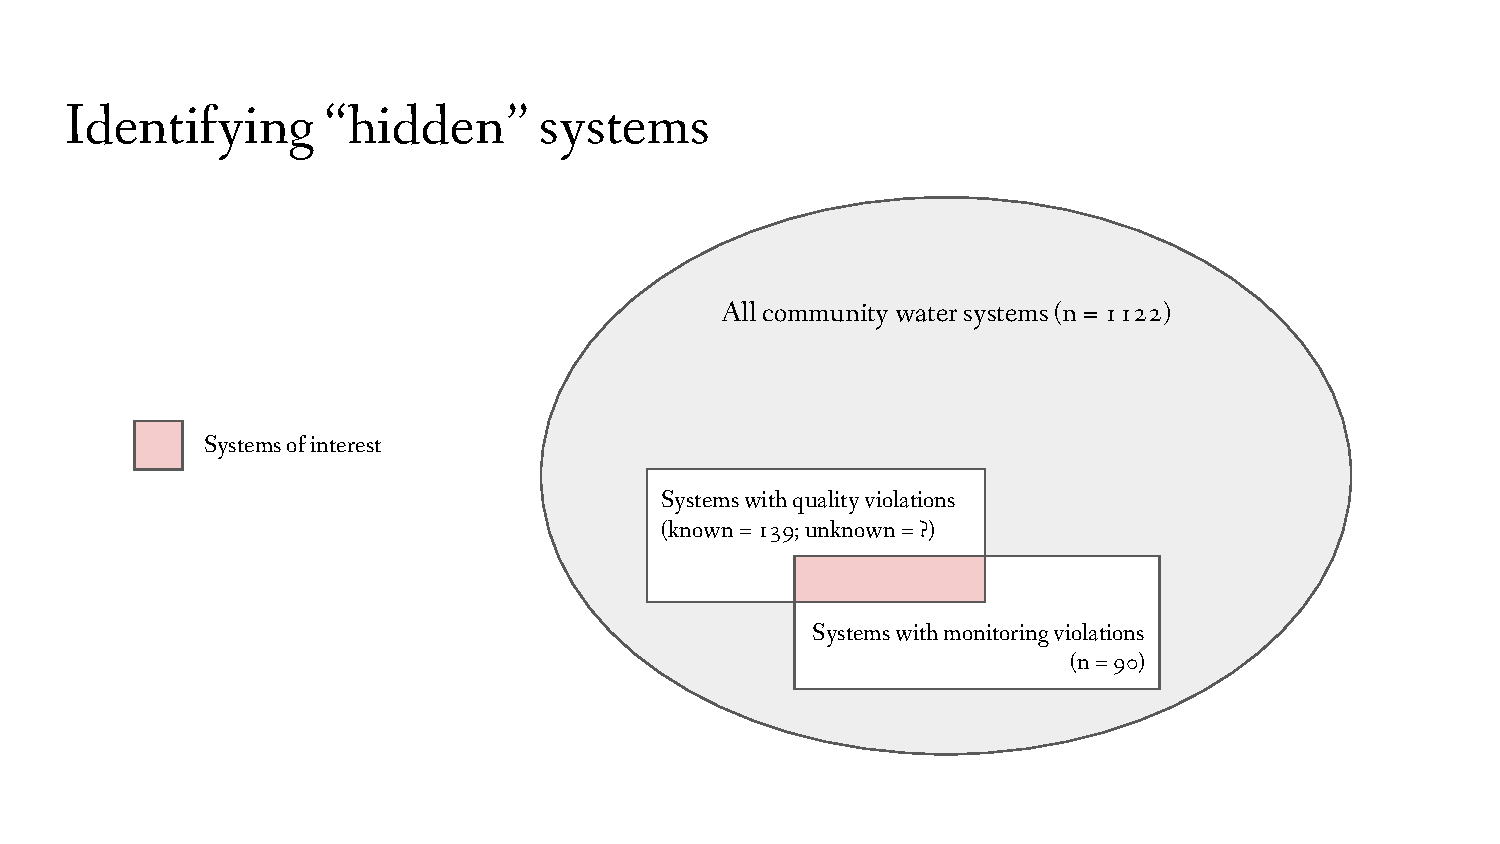
\includegraphics[width=1.1\textwidth]{seigi_8}
\end{frame}

\begin{frame}
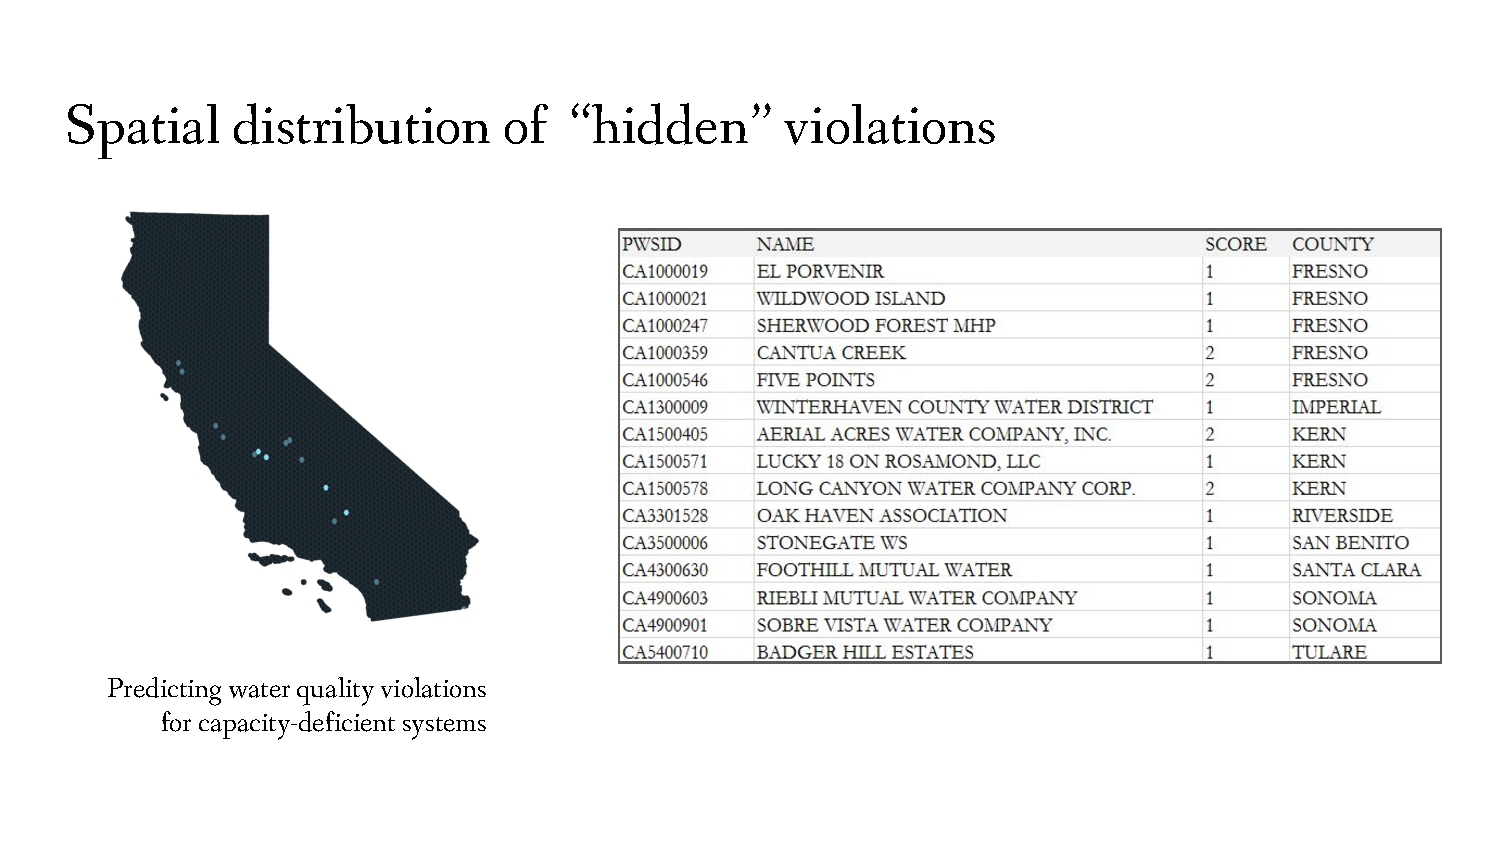
\includegraphics[width=1.1\textwidth]{seigi_9}
\end{frame}



\end{document}


